
\documentclass[11pt]{article}
\usepackage[%
  papersize={12.8cm,9.6cm},
  hmargin=1cm,%
  vmargin=1cm,%
  head=0.4cm,% might be changed later
  headsep=0pt,%
  foot=0.5cm% might be changed later
]{geometry}% http://ctan.org/pkg/geometry

\RequirePackage{amsmath}
\RequirePackage{amssymb}
\RequirePackage{amsthm}
%\RequirePackage{algorithmic}
%\RequirePackage{algorithm}
%\RequirePackage{theorem}
%\RequirePackage{eucal}
\RequirePackage{color}
\RequirePackage{url}
\RequirePackage{mdwlist}

\RequirePackage[all]{xy}
\CompileMatrices
\RequirePackage{hyperref}
\RequirePackage{graphicx}
\RequirePackage{relsize}


% xelatex:
\usepackage{fontspec}
\defaultfontfeatures{Ligatures=TeX}
%\usepackage[small,sf,bf]{titlesec}
%\setromanfont{DejaVu Serif}
%\setromanfont{Droid Serif}
%\setromanfont{Gentium} % nice! a bit fluffy
\setromanfont{Gentium Book Basic} % more bold



\RequirePackage{graphicx}
\usepackage{color}
\usepackage{amsfonts}


%\def\heading #1{\vskip 20pt \noindent\underline{\large \bf #1}\vskip 5pt}
\def\heading #1{\centerline{\underline{\bf\LARGE #1}}}
\def\vsp {\vskip 0.5cm}

\def\ket #1{|#1\rangle}
\def\bra #1{\langle#1|}
\def\braket #1#2{\langle#1|#2\rangle}

%\def\point {\vskip 5pt $\to$\ \ }
%\def\point {\vskip 5pt $\Longrightarrow$\ \ }
%\def\point {\vskip 5pt $\bigodot$\ \ }
\def\point {\vskip 5pt $\hookrightarrow$\ \ }

\def\N{\mathbb N}
\def\Z{\mathbb Z}
\def\R{\mathbb R}
\def\C{\mathbb C}
\def\tr{\triangleright}
\def\tensor{\otimes}


\begin{document}

\large

\pagenumbering{gobble}

%%%%%%%%%%%%%%%%%%%%%%%%%%%%%%%%%%%%%%%%%%%%%%%%%%%%%%%%%%%


\centerline{\LARGE }
\vskip 0.5cm
\centerline{\LARGE Distributivity, size, homomorphism}
\vskip 0.5cm
\centerline{\LARGE }

\vskip 1cm

\centerline{\Large Simon Burton}

\vskip 0.5cm

\centerline{School of Physics, The University of Sydney}


%\newpage %%%%%%%%%%%%%%%%%%%%%%%%%%%%%%%%%%%%%%%%%%%%%%%%%%
%
%\begin{center}
%\includegraphics[width=0.2\textwidth]{ExclamationMark.pdf}
%\end{center}
%
%\vskip 0.5cm
%\hspace{4 em} Possible \hspace{9 em} Actual
%

\newpage %%%%%%%%%%%%%%%%%%%%%%%%%%%%%%%%%%%%%%%%%%%%%%%%%%

\heading{Path counting}

\vsp
\centerline{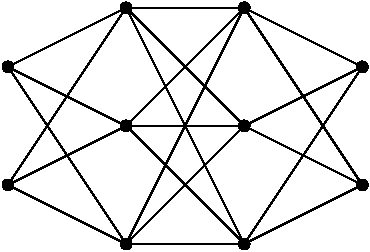
\includegraphics[]{pic-trellis.pdf}}
$$
    |\mbox{paths}| = 2.3.3.2 = 36
$$


\newpage %%%%%%%%%%%%%%%%%%%%%%%%%%%%%%%%%%%%%%%%%%%%%%%%%%

\heading{Path counting}

\vsp
\centerline{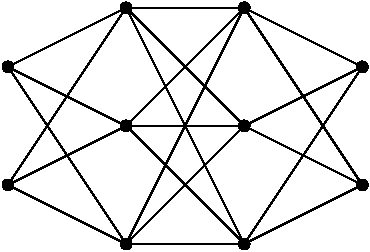
\includegraphics[]{pic-trellis.pdf}}
\begin{align*}
\begin{pmatrix}1&1&1\\1&1&1\end{pmatrix}
\begin{pmatrix}1&1&1\\1&1&1\\1&1&1\end{pmatrix}
\begin{pmatrix}1&1\\1&1\\1&1\end{pmatrix}
=\begin{pmatrix}9&9\\9&9\end{pmatrix}
\end{align*}
$$
    \sum_{jk} A_{ij} B_{jk} C_{kl}
    = \sum_{j} A_{ij} \sum_k B_{jk} C_{kl}
$$


\newpage %%%%%%%%%%%%%%%%%%%%%%%%%%%%%%%%%%%%%%%%%%%%%%%%%%

\heading{Path counting}

\vsp
\centerline{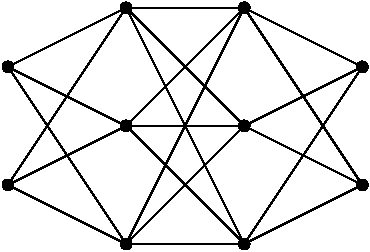
\includegraphics[]{pic-trellis.pdf}}

Distributivity:
$$
    a(b + c) = ab + ac
$$
\vsp\vsp
\vsp\vsp

\newpage %%%%%%%%%%%%%%%%%%%%%%%%%%%%%%%%%%%%%%%%%%%%%%%%%%

\heading{Minimum weight path}
\centerline{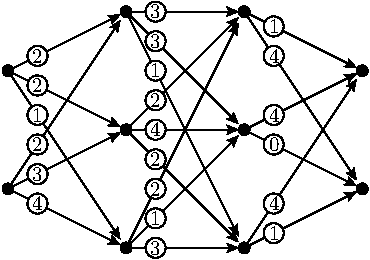
\includegraphics[]{pic-minpath-0.pdf}}
$$
    \min_{ijk} ( A_{ij} + B_{jk} + C_{kl} )
$$

\newpage %%%%%%%%%%%%%%%%%%%%%%%%%%%%%%%%%%%%%%%%%%%%%%%%%%

\heading{Minimum weight path}
\centerline{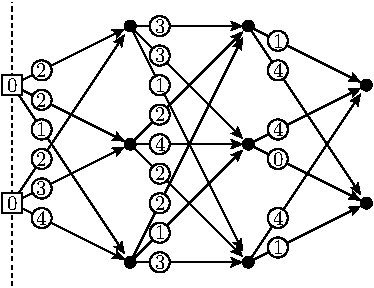
\includegraphics[]{pic-minpath-1.pdf}}

\newpage %%%%%%%%%%%%%%%%%%%%%%%%%%%%%%%%%%%%%%%%%%%%%%%%%%

\heading{Minimum weight path}
\centerline{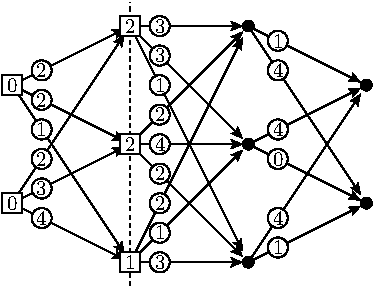
\includegraphics[]{pic-minpath-2.pdf}}

\newpage %%%%%%%%%%%%%%%%%%%%%%%%%%%%%%%%%%%%%%%%%%%%%%%%%%

\heading{Minimum weight path}
\centerline{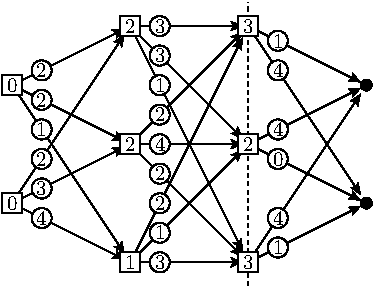
\includegraphics[]{pic-minpath-3.pdf}}

\newpage %%%%%%%%%%%%%%%%%%%%%%%%%%%%%%%%%%%%%%%%%%%%%%%%%%

\heading{Minimum weight path}
\centerline{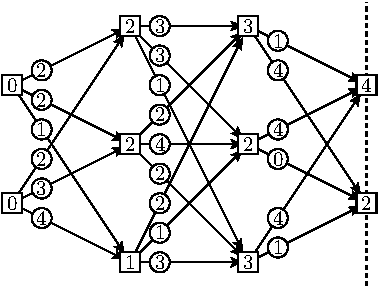
\includegraphics[]{pic-minpath-4.pdf}}
$$
    \min_{ijk} ( A_{ij} + B_{jk} + C_{kl} )
    = \min_k ( \min_j ( (\min_i A_{ij} ) + B_{jk} ) + C_{kl} )
$$

\newpage %%%%%%%%%%%%%%%%%%%%%%%%%%%%%%%%%%%%%%%%%%%%%%%%%%

\heading{Minimum weight path}
\centerline{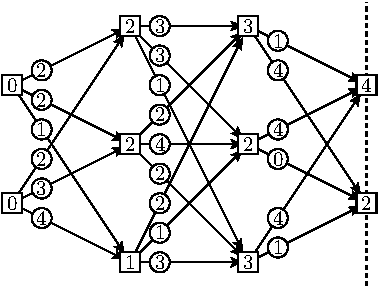
\includegraphics[]{pic-minpath-4.pdf}}

Distributivity:
$$
    a + \min(b, c) = \min(a+b, a+c)
$$

\newpage %%%%%%%%%%%%%%%%%%%%%%%%%%%%%%%%%%%%%%%%%%%%%%%%%%

\heading{Minimum weight path}
\centerline{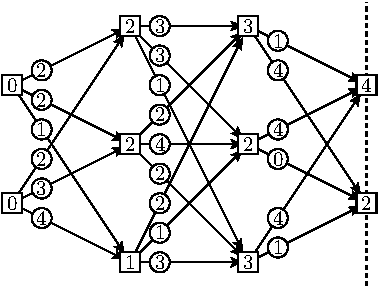
\includegraphics[]{pic-minpath-4.pdf}}

\vsp
... Bellman equation

... Hamilton-Jacobi equation


\newpage %%%%%%%%%%%%%%%%%%%%%%%%%%%%%%%%%%%%%%%%%%%%%%%%%%

\heading{Belief propagation}

\vsp
Joint probabilities factor as:
\begin{align*}
    p(x_1, x_2, x_3, x_4, x_5) = \ & p(x_1 | x_2, x_3, x_4, x_5)  p(x_2 | x_3, x_4, x_5) \\
        & \ \ \ p(x_3 | x_4, x_5) p( x_4 | x_5) p( x_5) 
\end{align*}

\newpage %%%%%%%%%%%%%%%%%%%%%%%%%%%%%%%%%%%%%%%%%%%%%%%%%%

\heading{Belief propagation}

\centerline{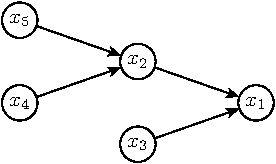
\includegraphics[]{pic-belief.pdf}}

\begin{align*}
    p(x_1 | x_2, x_3, x_4, x_5) &= p(x_1 | x_2, x_3) \\
    p(x_2 | x_3, x_4, x_5) &= p(x_2 | x_4, x_5)  \\
    p(x_3 | x_4, x_5)  &= p(x_3) \\
    p(x_4 | x_5) &= p(x_4)
\end{align*}

\newpage %%%%%%%%%%%%%%%%%%%%%%%%%%%%%%%%%%%%%%%%%%%%%%%%%%

%\begin{align*}
%    p(x_1, x_2, x_3, x_4, x_5) = p(x_1 | x_2, x_3)  p(x_2 | x_4, x_5) p(x_3) p(x_4) p( x_5) 
%\end{align*}
\heading{Belief propagation}
\centerline{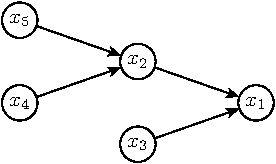
\includegraphics[]{pic-belief.pdf}}
\begin{align*}
    p(x_1) &= \sum_{x_1...x_5} p(x_1, x_2, x_3, x_4, x_5) \\
    &= \sum_{x_1...x_5} p(x_1 | x_2, x_3)  p(x_2 | x_4, x_5) p(x_3) p(x_4) p( x_5)  \\
    &= \sum_{x_1x_2x_3} p(x_1 | x_2, x_3)  p(x_3) \sum_{x_4 x_5} p(x_2 | x_4, x_5) p(x_4) p( x_5) 
\end{align*}

\newpage %%%%%%%%%%%%%%%%%%%%%%%%%%%%%%%%%%%%%%%%%%%%%%%%%%

\heading{Linear recurrence relations}

\vsp
For $n=1,2,...:$

$$
    a_{n+2} = a_{n+1} + a_n \ \ \mbox{with}\ \  a_1=1, a_2=1.
$$
\vsp
\vsp
\begin{verbatim}
def fibonacci(n):
    if n==1 or n==2:
        return 1
    return fibonacci(n-1) + fibonacci(n-2)
\end{verbatim}


\newpage %%%%%%%%%%%%%%%%%%%%%%%%%%%%%%%%%%%%%%%%%%%%%%%%%%

\heading{Linear recurrence relations}

\vsp
\centerline{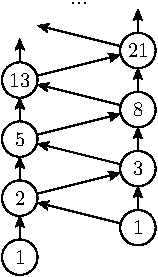
\includegraphics[]{pic-fibonacci.pdf}}
$$
    a_{n+2} = a_{n+1} + a_n \ \ \mbox{with}\ \  a_1=1, a_2=1.
$$


\newpage %%%%%%%%%%%%%%%%%%%%%%%%%%%%%%%%%%%%%%%%%%%%%%%%%%

\heading{Linear recurrence relations}

\vsp
\centerline{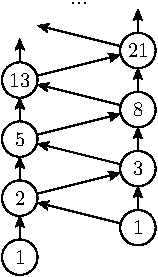
\includegraphics[]{pic-fibonacci.pdf}}
$$
    Sn := n+1
$$
$$
    f(SSn) = f(Sn) + f(n).
$$

\newpage %%%%%%%%%%%%%%%%%%%%%%%%%%%%%%%%%%%%%%%%%%%%%%%%%%

\heading{Perturbation theory}

\begin{align*}
    f(x) &= x^2 \sin(x) \\
    f'(x) &= 2x\cos(x) + x^2 \cos(x)
\end{align*}

Compute to first order:
\begin{align*}
    f(x+\varepsilon) &= (x+\varepsilon)^2 \sin(x+\varepsilon)
\end{align*}
with $\varepsilon^2 = 0.$


\newpage %%%%%%%%%%%%%%%%%%%%%%%%%%%%%%%%%%%%%%%%%%%%%%%%%%

\heading{Automatic differentiation}

\centerline{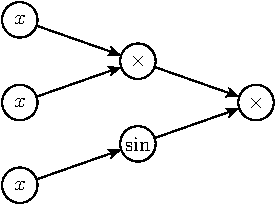
\includegraphics[]{pic-diff.pdf}}

Chain rule:
\begin{align*}
    D(f\circ g)(x) = Df(g(x))\cdot Dg(x)
\end{align*}

... neural networks

\newpage %%%%%%%%%%%%%%%%%%%%%%%%%%%%%%%%%%%%%%%%%%%%%%%%%%

\heading{Renormalization}

\vsp
Classical spin chain: $H = \sum_{i=1}^N \sigma_i\sigma_{i+1}$ 
\begin{align*}
    Z &= \sum_{\sigma_1...\sigma_N} \exp\Bigl( \sum_{i=1}^N \sigma_i\sigma_{i+1} \Bigr) 
       = \sum_{\sigma_1...\sigma_N} \prod_{i=1}^N  \exp\bigl( \sigma_i\sigma_{i+1} \bigr) \\
      &= \sum_{\sigma_1\sigma_3...} \ \prod_{i=2,4...} \Bigl(
        \sum_{\sigma_i} \exp\bigl( \sigma_i\sigma_{i+1} \bigr) \Bigr) \\
\end{align*}
%where is the path integral?

\newpage %%%%%%%%%%%%%%%%%%%%%%%%%%%%%%%%%%%%%%%%%%%%%%%%%%

\heading{Sum over paths}

\begin{align*}
\frac{d}{dt} \psi(t) = H f(t)
\end{align*}
has solution:
\begin{align*}
\psi(t) &= \exp(tH) \\
  &= \sum_{n} \frac{1}{n!} t^n H^n
\end{align*}

\newpage %%%%%%%%%%%%%%%%%%%%%%%%%%%%%%%%%%%%%%%%%%%%%%%%%%

\heading{Sum over paths}

\vsp
$$
\exp(H) = 1 + H + \frac{1}{2}H^2 + ... + \frac{1}{n!} H^n + ...
$$
\vsp
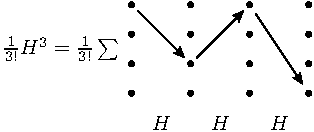
\includegraphics[width=0.8\textwidth]{pic-exp.pdf}


\newpage %%%%%%%%%%%%%%%%%%%%%%%%%%%%%%%%%%%%%%%%%%%%%%%%%%

\heading{Quantum}
\vsp
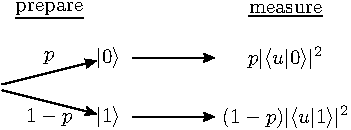
\includegraphics[width=0.8\textwidth]{pic-quantum.pdf}

\newpage %%%%%%%%%%%%%%%%%%%%%%%%%%%%%%%%%%%%%%%%%%%%%%%%%%

\heading{Quantum}
\vsp
\centerline{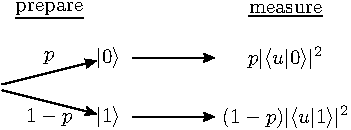
\includegraphics[width=0.7\textwidth]{pic-quantum.pdf}}
\vsp
\begin{align*}
&p|\braket{u}{0}|^2 + (1-p)|\braket{u}{1}|^2 \\
=& \bra{u}\Bigl( p\ket{0}\bra{0} + (1-p)\ket{1}\bra{1} \Bigr ) \ket{u}
\end{align*}

\newpage %%%%%%%%%%%%%%%%%%%%%%%%%%%%%%%%%%%%%%%%%%%%%%%%%%

\heading{Quantum}
\vsp
\centerline{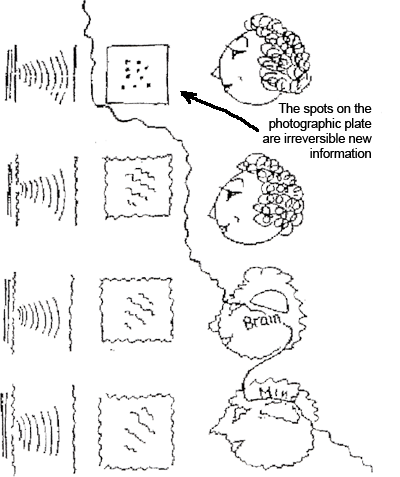
\includegraphics[width=0.5\textwidth]{Bell.png}}

\newpage %%%%%%%%%%%%%%%%%%%%%%%%%%%%%%%%%%%%%%%%%%%%%%%%%%

\heading{Size}
\vsp
\begin{align*}
    \mu(A\cup B) &= \mu(A) + \mu(B)
\end{align*}

\newpage %%%%%%%%%%%%%%%%%%%%%%%%%%%%%%%%%%%%%%%%%%%%%%%%%%

\heading{Size}
\vsp
\begin{align*}
    \mu(A\cup B) &= \mu(A) + \mu(B) - \mu(A\cap B)
\end{align*}

\newpage %%%%%%%%%%%%%%%%%%%%%%%%%%%%%%%%%%%%%%%%%%%%%%%%%%

\heading{Size}
\vsp
\begin{align*}
    \mu(A\cup B) &= \mu(A) + \mu(B) - \mu(A\cap B) \\
    \chi(X\cup Y) &= \chi(X) + \chi(Y) - \chi(X\cap Y) \\
    H(p, q) &= H(p) + H(q) - I(p:q) \\
\end{align*}

\newpage %%%%%%%%%%%%%%%%%%%%%%%%%%%%%%%%%%%%%%%%%%%%%%%%%%

\heading{Size}
\vsp
\begin{align*}
\mu(A\cup B\cup C) = \ &\mu(A) + \mu(B) + \mu(C)  \\
                     &- \mu(A\cap B) - \mu(A\cap C) - \mu(B\cap C) \\
                     &+ \mu(A\cap B \cap C)
\end{align*}


\newpage %%%%%%%%%%%%%%%%%%%%%%%%%%%%%%%%%%%%%%%%%%%%%%%%%%

\heading{Convexity}
\vsp

Consider a convex combination 
$$ \alpha a + (1-\alpha) b$$ 
for $a,b\in\R^n.$
We have:
\begin{align*}
    x + \bigl( \alpha a + (1-\alpha) b \bigr) = \alpha (x + a) + (1-\alpha) (x + b)
\end{align*}

\newpage %%%%%%%%%%%%%%%%%%%%%%%%%%%%%%%%%%%%%%%%%%%%%%%%%%

\heading{Convexity}
\vsp

Define:
$$
    a+_\alpha b := \alpha a + (1-\alpha) b
$$

then
\begin{align*}
    x + ( a +_\alpha b ) = (x+a) +_\alpha (x+b).
\end{align*}

\newpage %%%%%%%%%%%%%%%%%%%%%%%%%%%%%%%%%%%%%%%%%%%%%%%%%%

\heading{Convexity}
\vsp

Define:
$$
    a+_\alpha b := \alpha a + (1-\alpha) b
$$

then
\begin{align*}
    x + ( a +_\alpha b ) = (x+a) +_\alpha (x+b).
\end{align*}

And more:
\begin{align*}
    x +_\alpha ( a +_\beta b ) = (x+_\alpha a) +_\beta (x+_\alpha b).
\end{align*}


\newpage %%%%%%%%%%%%%%%%%%%%%%%%%%%%%%%%%%%%%%%%%%%%%%%%%%

\heading{Conjugation}
\vsp

Given a group $G$
with elements $g, h, k$
define 
$$g\tr h := g^{-1} h g.$$
Then we have
$$
g \triangleright (h \triangleright k) = (g\triangleright h)\triangleright(g\triangleright k).
$$

\newpage %%%%%%%%%%%%%%%%%%%%%%%%%%%%%%%%%%%%%%%%%%%%%%%%%%

\heading{Yang-Baxter equation}
\vsp

$$(R\tensor I) (I\tensor R) (R\tensor I) = (I\tensor R) (R\tensor I) (I\tensor R)$$
%Also the Jacobi identity fits here.
\vsp
\centerline{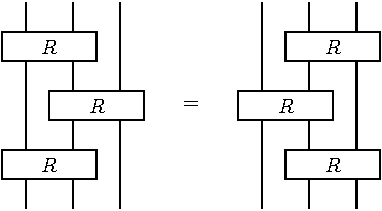
\includegraphics[]{pic-yb.pdf}}


\newpage %%%%%%%%%%%%%%%%%%%%%%%%%%%%%%%%%%%%%%%%%%%%%%%%%%

\heading{Yang-Baxter equation}
\vsp
$$\sigma_1 \sigma_2 \sigma_1 = \sigma_2 \sigma_1 \sigma_2.$$
\vsp
\centerline{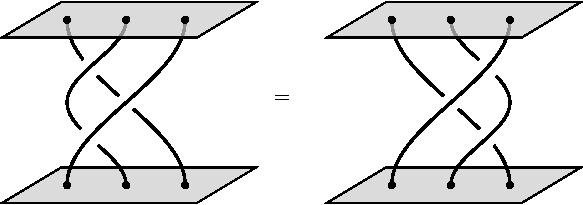
\includegraphics[]{pic-braid.pdf}}


\newpage %%%%%%%%%%%%%%%%%%%%%%%%%%%%%%%%%%%%%%%%%%%%%%%%%%

\heading{Yang-Baxter equation}
\vsp
\centerline{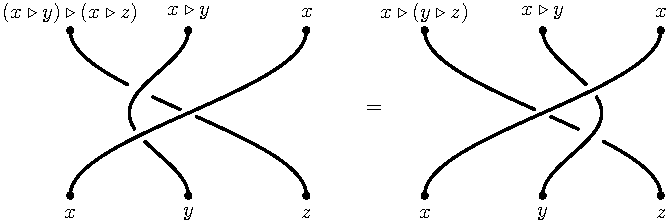
\includegraphics[]{pic-braid-shelf.pdf}}

\newpage %%%%%%%%%%%%%%%%%%%%%%%%%%%%%%%%%%%%%%%%%%%%%%%%%%

\centerline{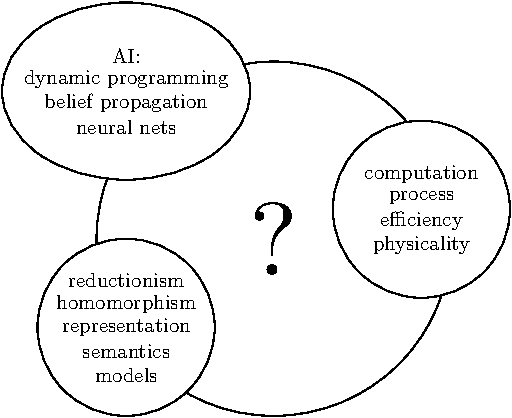
\includegraphics[]{pic-question.pdf}}

\end{document} %%%%%%%%%%%%%%%%%%%%%%%%%%%%%%%%%%%%%%%%%%%%%%%%%%%%%%%%%%%

